\documentclass{exam}
\usepackage[utf8]{inputenc}
\usepackage{lmodern}
\usepackage{microtype}

% \usepackage[parfill]{parskip}
\usepackage[dvipsnames]{xcolor}
\usepackage{amsmath}
\usepackage{amsfonts}
\usepackage{amsthm}
\usepackage{siunitx}
\DeclareSIUnit\year{yr}
\DeclareSIUnit\foot{ft}
\DeclareSIUnit\litre{\liter}

\usepackage{skull}

\usepackage{pgfplots}
\usepgfplotslibrary{polar}
\pgfplotsset{compat=1.11}
\usepgfplotslibrary{statistics}
\usepackage{graphicx}
\usepackage{sidecap}
\sidecaptionvpos{figure}{c}
\usepackage{float}
\usepackage{gensymb}
\usepackage{tkz-euclide}
\usetkzobj{all}
\usepackage{commath}
\usepackage{hyperref}
\usepackage{enumitem}
\usepackage{wasysym}
\usepackage{multicol}
\usepackage{mathtools}
\usepackage{tcolorbox}
\usepackage{tabularx}
\usepackage[version=4]{mhchem}
\usepackage{changepage}
\usepackage{listings}
\lstset{basicstyle=\ttfamily\linespread{0.8}\small}

\renewcommand*{\thefootnote}{\fnsymbol{footnote}}

\newtheorem*{thm}{Theorem}
\newtheorem*{iden}{Identity}
\newtheorem*{lemma}{Lemma}
\newtheorem{obs}{Observation}
\theoremstyle{definition}
\newtheorem*{defn}{Definition}
\newtheorem*{ex}{Example}
\newtheorem{con}{Construction}
\newtheorem*{alg}{Algorithm}

\newtheoremstyle{break}
  {\topsep}{\topsep}%
  {\itshape}{}%
  {\bfseries}{}%
  {\newline}{}%
\theoremstyle{break}
\newtheorem*{bthm}{Theorem}

% russian integral
\usepackage{scalerel}
\DeclareMathOperator*{\rint}{\scalerel*{\rotatebox{17}{$\!\int\!$}}{\int}}

% \DeclareMathOperator*{\rint}{\int}

\pgfplotsset{vasymptote/.style={
    before end axis/.append code={
        \draw[densely dashed] ({rel axis cs:0,0} -| {axis cs:#1,0})
        -- ({rel axis cs:0,1} -| {axis cs:#1,0});
    }
}}

% \pointsinrightmargin
\boxedpoints
\pointname{}

\newcommand{\questioA}{\question[\texttt{\textbf{\color{Cerulean} A}}]}
\newcommand{\questioM}{\question[\texttt{\textbf{\color{PineGreen} M}}]}
\newcommand{\questioE}{\question[\texttt{\textbf{\color{WildStrawberry} E}}]}
\newcommand{\questioS}{\question[\texttt{\textbf{\color{Goldenrod} S}}]}
\newcommand{\questioO}{\question[\texttt{\textbf{\color{BurntOrange} O}}]}

\newcommand{\parA}{\part[\texttt{\textbf{\color{Cerulean} A}}]}
\newcommand{\parM}{\part[\texttt{\textbf{\color{PineGreen} M}}]}
\newcommand{\parE}{\part[\texttt{\textbf{\color{WildStrawberry} E}}]}
\newcommand{\parS}{\part[\texttt{\textbf{\color{Goldenrod} S}}]}
\newcommand{\parO}{\part[\texttt{\textbf{\color{BurntOrange} O}}]}

\newcommand{\subparA}{\subpart[\texttt{\textbf{\color{Cerulean} A}}]}
\newcommand{\subparM}{\subpart[\texttt{\textbf{\color{PineGreen} M}}]}
\newcommand{\subparE}{\subpart[\texttt{\textbf{\color{WildStrawberry} E}}]}
\newcommand{\subparS}{\subpart[\texttt{\textbf{\color{Goldenrod} S}}]}
\newcommand{\subparO}{\subpart[\texttt{\textbf{\color{BurntOrange} O}}]}

\newcommand{\mainHeader}[2]{\section*{NCEA Level 2 Mathematics\\#1. #2}}
\newcommand{\mainHeaderHw}[2]{\section*{NCEA Level 2 Mathematics (Homework)\\#1. #2}}
\newcommand{\seealso}[1]{\begin{center}\emph{See also #1.}\end{center}}
\newcommand{\drills}[1]{\begin{center}\emph{Drill problems: #1.}\end{center}}
\newcommand{\basedon}[1]{\begin{center}\emph{Notes largely based on #1.}\end{center}}


\begin{document}

\mainHeader{12}{Tangent Lines and Approximations}
One application of calculus is to find approximations to curves. Our goal is to write
down a linear equation that approximates any given curve (around a given point). This is
useful if (for example) we are given a complicated function like
\begin{displaymath}
  f(x) = [\sin(x^{100})]^{[\cos(\sin x^2)]}.
\end{displaymath}
This function is so weird that the graphing software I use cannot even graph it properly. The
value of this function at $ x = 0 $ is very easy to calculate:
\begin{displaymath}
  f(0) = [\sin(0^{100})]^{[\cos(\sin 0^2)]} = 0^{\cos(0)} = 0
\end{displaymath}
However, as soon as we try to calculate other values it becomes difficult.

Suppose we want to know the value of a function near a point that it's easy to find the value of
the function at --- for example, $ f(0.001) $. Our goal is to to draw the line through the easy
point, with the same slope as the function at that point, and then work out what our desired $ x$-value
maps to using this easy function.

\begin{defn}
  Let $ y = f(x) $ be a curve, and let $ f $ be differentiable at some $ x$-value $ x_0 $. Then
  the \emph{tangent line} to the curve at $ x_0 $ is simply the line through the point $ (x_0, f(x_0)) $
  that has the same slope as the curve at that point.

  From our work on coordinate geometry, we know that the equation of this line is
  \begin{displaymath}
    y - f(x_0) = f'(x_0)(x - x_0).
  \end{displaymath}
\end{defn}

Let's take an example.

\begin{ex}
  Let us calculate $ \sqrt{4.03} $ by hand(!). If we consider the function $ f(x) = \sqrt{4 + x} $,
  then $ \sqrt{4.03} = f(0.03) $. Let's draw the situation out:
  \begin{center}
    \begin{tikzpicture}
      \begin{axis}[
        axis lines = center,
        xlabel = $ x $,
        ylabel = {$ y $}
      ]
        \addplot[domain = -4:6, color = green, samples=100] {sqrt(4+x)};
        \draw[color=red] (0.03,0) -- (0.03,4);
        \node[label=left:{\color{red}$ x = 0.03 $}] at (2.4,1.5) {};
        \node[label=above:{\color{green}$ y = \sqrt{4 + x} $}] at (-2.2, 1.6) {};
      \end{axis}
    \end{tikzpicture}
  \end{center}
  So we want the tangent line to $ f $ at the point $ x = 0 $. We have that $ f'(x) = \frac{1}{2\sqrt{4 + x}} $ (why? we can easily
  take the derivative of $ \sqrt{x} $, it's just $ \frac{1}{2\sqrt{x}} $ --- and the graph of $ f $ is just the graph of $ \sqrt{x} $
  but shifted four units to the left, so we just shift the slope function itself four units to the left to match up),
  and so $ f'(0) = \frac{1}{4} $. The tangent line is the line through $ (0, f(0)) = (0, 2) $ with gradient $ \frac{1}{4} $,
  which has equation
  \begin{displaymath}
    y - 2 = \frac{1}{4}x.
  \end{displaymath}
  Hence $ \sqrt{4.03} \approx \frac{1}{4} \times 0.03 + 2 = 2.0075 $ --- and, as promised, all of these calculations
  can be done without a calculator. (According to my calculator, $ \sqrt{4.03} \approx 2.007486 $ and so we are not far
  off at all.)
\end{ex}

Now, with all the motivation out of the way, we will just look at some more simple examples.
\begin{ex}
  Consider $ y = x^2 $. At $ (2,4) $, the tangent line has slope 4 and hence equation $ y - 4 = 4(x - 2) $:
  \begin{center}
    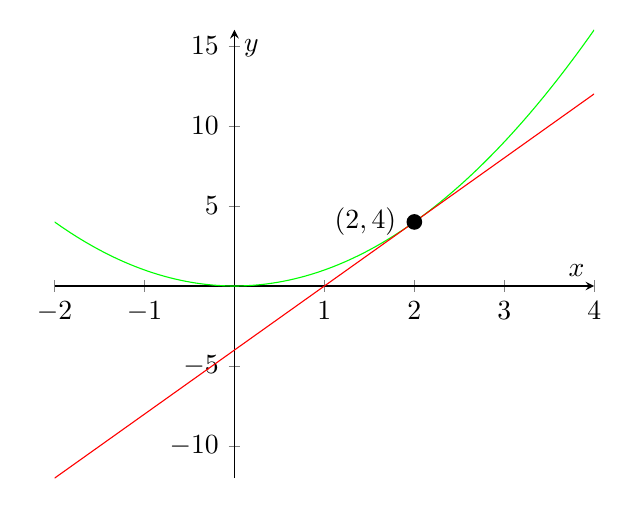
\begin{tikzpicture}
      \begin{axis}[
        axis lines = center,
        xlabel = $ x $,
        ylabel = {$ y $}
      ]
        \addplot[domain = -2:4, color = green, samples=100] {x^2};
        \addplot[domain = -2:4, color = red, samples=100] {4*(x - 2) + 4};
        \node[label=left:{$ (2,4) $},circle,fill,inner sep=2pt] at (2,4) {};
      \end{axis}
    \end{tikzpicture}
  \end{center}
\end{ex}

\begin{ex}
  Consider $ y = x^3 - 2x^2 - x + 1 $. At $ (3,7) $, the tangent line has slope 14 and hence equation $ y - 7 = 14(x - 3) $:
  \begin{center}
    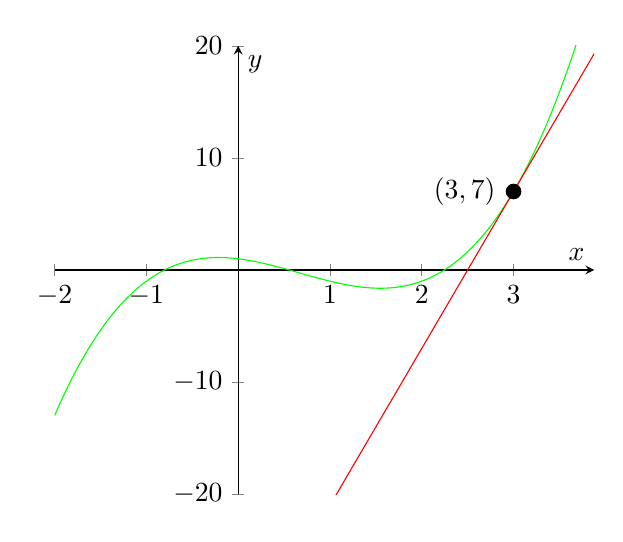
\begin{tikzpicture}
      \begin{axis}[
        axis lines = center,
        xlabel = $ x $,
        ylabel = {$ y $},
        ymin = -20,ymax = 20
      ]
        \addplot[domain = -2:4, color = green, samples=100] {x^3 - 2*x^2 - x + 1};
        \addplot[domain = -2:4, color = red, samples=100] {14*(x - 3) + 7};
        \node[label=left:{$ (3,7) $},circle,fill,inner sep=2pt] at (3,7) {};
      \end{axis}
    \end{tikzpicture}
  \end{center}
\end{ex}

\begin{ex}
  Consider $ y = \frac{1}{2x^2} - 1 $. At $ (1, -1/2) $, the tangent line has slope $-1$ and hence equation $ y + 1/2 = -(x - 1) $:
  \begin{center}
    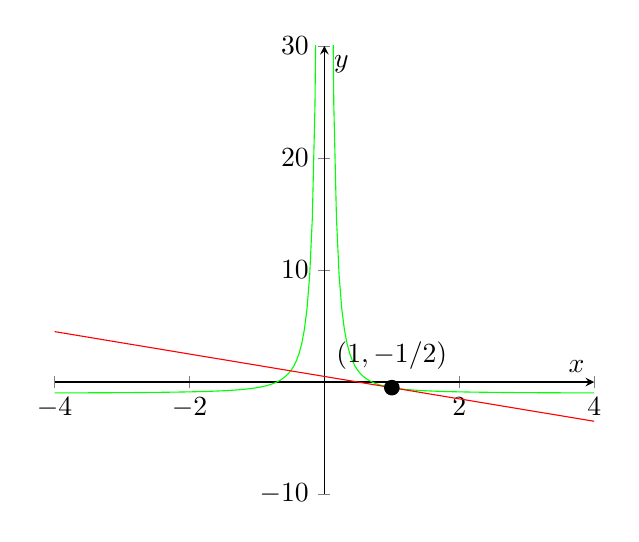
\begin{tikzpicture}
      \begin{axis}[
        axis lines = center,
        xlabel = $ x $,
        ylabel = {$ y $},
        ymax = 30, ymin = -10
      ]
        \addplot[domain = 0.1:4, color = green, samples=100] {1/(2*x^2) - 1};
        \addplot[domain = -4:-0.1, color = green, samples=100] {1/(2*x^2) - 1};
        \addplot[domain = -4:4, color = red, samples=100] {-1*(x - 1) - 0.5};
        \node[label=above:{$ (1,-1/2) $},circle,fill,inner sep=2pt] at (1,-1/2) {};
      \end{axis}
    \end{tikzpicture}
  \end{center}
\end{ex}

\subsection*{Questions}
\begin{questions}
  \question Why is there no tangent line to $ y = x^2 $ at the point $ (0, -1) $?
  \question Consider the function $ f(x) = 7x^3 + 2x $.
    \begin{center}\begin{tikzpicture}
      \begin{axis}[
        scale = .8,
        axis lines = center,
        xlabel = $ x $,
        ylabel = {$ y $}
      ]
        \addplot[domain = 0:4, color = green, samples=100] {7*x^3 + 2*x};
        \addplot[domain = 0:4, color = red, samples=100] {86*(x - 2) + 60};
      \end{axis}
    \end{tikzpicture}\end{center}
    \begin{parts}
      \part What is the slope of the graph of $ y = f(x) $ around $ x = 2 $?
      \part Give the equation of the tangent line to the graph at $ x = 2 $.
    \end{parts}
  \question Consider the function $ g(x) = 2x^2 + \frac{3}{x} $.
    \begin{center}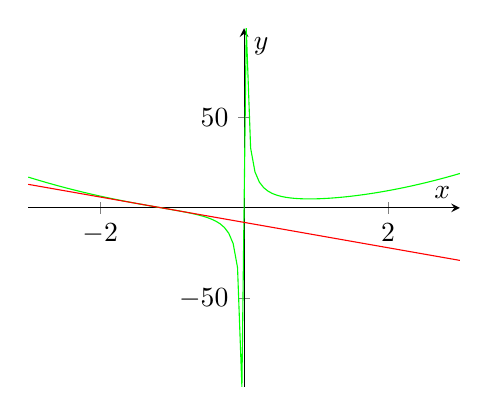
\begin{tikzpicture}
      \begin{axis}[
        scale = .8,
        xmin = -3, xmax = 3,
        axis lines = center,
        xlabel = $ x $,
        ylabel = {$ y $}
      ]
        \addplot[domain = -3:3, color = green, samples=100] {2*x^2 + 3/x};
        \addplot[domain = -3:3, color = red, samples=100] {-7*(x + 1) -1};
      \end{axis}
    \end{tikzpicture}\end{center}
    \begin{parts}
      \part What is the slope of the graph of $ y = g(x) $ around $ x = -1 $?
      \part Give the equation of the tangent line to the graph at $ x = -1 $.
      \part The normal line to a graph at a point is the line going through that point that lies at right angles to the graph (and hence to the
            tangent line to the graph).
        \begin{subparts}
          \subpart Consider the line with slope $ m $ going through $ (x_0, y_0) $; it has equation $ (y - y_0) = m(x - x_0) $. What
                   is the slope of the line at right angles to it going through the same point?
          \subpart Give the equation of the normal line to the graph of $ y = g(x) $ at $ x = -1 $.
        \end{subparts}
    \end{parts}
  \question
    \begin{parts}
      \part Find the slope function of $ y = x^3 + 8x^2 + 22x - 21 $ in two different ways:
        \begin{subparts}
          \subpart By rewriting the function as $ y = (x - 3)^3 + (x - 3)^2 + (x - 3) $ and then differentiating $ z^3 + z^2 + z $;
          \subpart By simply taking the derivative of the original function in its expanded form.
        \end{subparts}
      \part Hence explain how the derivative $ \od{y}{x} $ is related geometrically to the derivative $ \od{}{z}[z^3 + z^2 + z] $.
      \part Show that there are no points where the graph of $ y $ versus $ x $ has a horizontal tangent line.
    \end{parts}
  \question To expand slightly on the previous question, consider now the graph $ y = (x^2 + 1)^2 + (x^2 + 1) $.
    \begin{parts}
      \part By expanding the brackets, find $ \od{y}{x} $.
      \part Show that $ \od{y}{x} \neq 2(x^2 + 1) + 1 $. (Where did this right-hand function come from?)
      \part Can you explain why our argument about `shifting functions' does not work here? Hint: if we transform
            $ x $ to $ x - 3 $, there is no shrinking or stretching going on --- but this is not always the case.
    \end{parts}
  \question A function $ f $ is differentiable at a point $ x $ if the value $ f'(x) $ is well-defined.
    \begin{parts}
      \part Give some examples of functions which are \emph{not} differentiable at some point.
      \part Can you define differentiability in a different way, using tangent lines?
      \part Is it ever possible for a function to have a horizontal normal line at any point? Explain how your answer is related
            to the idea of differentiability.
    \end{parts}
  \question Consider the hyperbola $ y = 1/x $.
    \begin{parts}
      \part Explain why the hyperbola has no tangent line at $ x = 0 $.
      \part Show that the tangent lines to the hyperbola at $ (-1,-1) $ and $ (1,1) $ are parallel.
      \part More generally, show that the tangent lines to the hyperbola at $ (-x, -1/x) $ and $ (x, 1/x) $ are always parallel.
      \part Are there any points on the hyperbola which share a common normal line (not simply a normal line with the same slope,
            but the same line full stop)? What about tangent lines? Hint: yes, and no.
    \end{parts}
  \question Finally, here are some functions and points to find tangent lines at. If there is no tangent line at the point given,
            carefully explain why. Draw some graphs out as well.
    \begin{parts}
      \part $ y = 3x^2 + 3x + 1 $ at $ (0, 1) $.
      \part $ y = \sqrt{1 - x^2} $ at $ (1, 0) $.
      \part $ y = 1/x^2 $ at $ (1,1) $.
      \part $ y = 1/x^2 $ at $ (2,1/4) $.
      \part $ y = \sqrt[4]{x^3} $ at $ (2, \sqrt[4]{8}) $.
      \part $ y = \sqrt[3]{x^2 + 2x + 1} $ at $ (0, 1) $.(Hint: complete the square.)
    \end{parts}
\end{questions}

\end{document}
